\documentclass[conference]{IEEEtran}
%\IEEEoverridecommandlockouts
% The preceding line is only needed to identify funding in the first footnote. If that is unneeded, please comment it out.
\usepackage{cite}
\usepackage{amsmath,amssymb,amsfonts}
\usepackage{algorithmic}
\usepackage{graphicx}
\usepackage{textcomp}
\usepackage{xcolor}
\usepackage{subcaption}
\def\BibTeX{{\rm B\kern-.05em{\sc i\kern-.025em b}\kern-.08em
    T\kern-.1667em\lower.7ex\hbox{E}\kern-.125emX}}
\begin{document}

\title{
    XAI: Explainable Neural Network Recognition of Handwritten Characters
}

\author{\IEEEauthorblockN{Author 1}
\IEEEauthorblockA{\textit{dept. name of organization (of Aff.)} \\
\textit{name of organization (of Aff.)}\\
City, Country \\
email address}
\and
\IEEEauthorblockN{Author 2}
\IEEEauthorblockA{\textit{dept. name of organization (of Aff.)} \\
\textit{name of organization (of Aff.)}\\
City, Country \\
email address}
\and
\IEEEauthorblockN{Author 3}
\IEEEauthorblockA{\textit{dept. name of organization (of Aff.)} \\
\textit{name of organization (of Aff.)}\\
City, Country \\
email address}
}

\maketitle

\begin{abstract}
    The prevalence of Artificial Intelligence (AI) in many aspects of life has
    brought about increasing concern and desire for explainability.  This work poses
    and outlines the implementation of an Explainable Artificial Intelligence data
    pipeline, comprised of Neural Networks, for recognition of handwritten
    characters in the EMNIST database. A key challenge for supervised learning and
    explainability is ambiguous and mislabeled samples in training data.  Techniques
    are applied to identify some of the issues with ambiguous and mislabeled data in
    EMNIST.  This paper introduces a neural network architecture which recognizes
    handwritten characters and produces explanations based on a character property
    analysis.  A key concept to explainability that is introduced here is correctly
    pruning the training set in order to improve the explainability and avoid
    misleading training set labels. The neural network architecture is used to
    resolve some of the training set issues by leveraging classifications and
    explanations. Results from the EMNIST character database are provided.
\end{abstract}

\begin{IEEEkeywords}
    Explainable Artificial Intelligence, XAI, Neural Network, Machine Learning, Training Set Pruning
\end{IEEEkeywords}

\section{Introduction}
Artificial Intelligence (AI), especially Machine Learning (ML) has been used
widely in recent years.  Many aspects of human interaction with technology may
involve AI e.g, digital assistants, online shopping, and autonomous vehicles.

While modern ML systems have been very successful in many tasks, there has been
a lack of an ability to explain decisions made by a ML system. ML systems
largely act as an opaque box.  The activity that occurs within the box is hidden
to humans.  When AI is used in making important decisions there is a strong
desire to explain why a decision was made.  Some proposed legislation suggests
that an explanation, suitable for a human, must be provided in decisions made
by automated systems.  Explainable Artificial Intelligence (XAI) has been a keen
area of interest to DARPA\cite{Gunning_Aha_2019} as well.

Handwritten sample datasets, such as the Modified National Institute of
Standards and Technology database (MNIST)\cite{deng2012mnist}, which consists of
70,000 samples of handwritten digits, and the Extended MNIST database\cite{cohen2017emnist}
(EMNIST), which contains over 800,000 samples, serve as
important datasets that have been utilized widely in ML to evaluate models. The
datasets are valuable testbeds to leverage for research. Despite the wide use of
MNIST and EMNIST, there are problems with samples that are ambiguous or
mislabeled.  These ambiguous and mislabeled samples are especially challenging
for explainability.

A property-based XAI methodology\cite{whitten21} that provides rationale for
classification decisions was recently introduced.  In this methodology,
explainable properties, transformations of data related to properties, and ML
models trained against those property transformations are used to make local
classification decisions.  The local, property-based, decisions then contribute
to a global classification.  The properties that were used in the global
classification contribute rationale for the decision.  This methodology achieved
acceptable accuracy results using MNIST and was able to provide explanations
related to properties of the samples.

This work constructs an XAI data pipeline from the concepts of the
property-based XAI methodology and attempts to improve on past results by
leveraging more modern ML models.  This work also applies the pipeline to the
expansive EMNIST dataset to produce promising results.  Finally, issues with the
training sets are identified and the pipeline is used in an attempt to resolve
the issues using classifications and explainability from the pipeline.

%% motivation
\subsection{Motivation}

Current Neural Networks (NN) and ML models do not explain or justify decisions
in a manner suitable to present to a human user.  There is currently no
algorithm that can take weights of NN and justify decisions to a human.

This work seeks to improve on a Property-Based XAI methodology and construct an
explainable data pipeline. The aim is to increase recognition accuracy while
providing a human understandable explanation for decision.

An expanded dataset of handwritten characters, EMNIST, is utilized. This work
also outlines the experiences and challenges of the expanded dataset. A key
challenge in explainability is resolving ambiguous and mislabeled samples in the
expanded dataset.  Label issues in the EMNIST dataset are identified the
explainable pipeline is leveraged in an attempt to resolve the issues.

\section{Related Work}

\subsection{Neural Networks}

Since the presentation of the McCulloch-Pitts neuron
model\cite{McCulloch1943-MCCALC-5} in 1943 and the subsequent implementation of
the perceptron\cite{rosenblatt1957perceptron}, neural network models, tools, and
hardware has improved drastically, e.g., backpropagation\cite{6795724},
Convolutional Neural Networks (CNN)\cite{fukushima1982neocognitron}, gradient
based learning\cite{726791}, deep residual learning\cite{7780459}.  In this work
CNNs and Resnet are utilized and compared.

\subsection{Explainable Artificial Intelligence}

The ability to map the learning classifier or recognizer to human-based
explainability is a challenging task for human understandability.  Currently,
there are at least seventeen explainable techniques such as decision tree-based,
rule-based (i.e. knowledgebase), salience mapping, sensitivity-based analysis,
feature importance, fuzzy-based, neural-network, and genetic-programming based.
These techniques use one of three basic evaluation approaches:
application-grounded, human-grounded and functionally grounded
\cite{Arrieta2020ExplainableAI,Survey18,Fuzzy19,Hagras18,GP18}.


There has been some work done in a systematic review of XAI
\cite{vilone2020explainable}.  The XAI methodology from \cite{whitten21} took a
knowledge-based approach to construct a classification system with intrinsic
explainability.  The method involves manually discovering multiple properties
across classes of input that contribute to explainability.  Transforms related
to properties were identified and applied to alter inputs.  Granular property
based inferencing is used to support a global decision.  Output from the
property-based methodology is a textual justification for the decision
based upon the explainable properties.

\subsection{EMNIST}

The Extended MNIST (EMNIST)\cite{cohen2017emnist} character and digit dataset
consists of over 800,000 28x28 images of handwritten characters.  The dataset is
split in six different ways, based on classes included and the balancing of
classes in each split.  The split primarily used in this work is the EMNIST
balanced data set which contains 131,600 samples in 46 classes consisting of
decimal digits, 26 uppercase letters, and 10 lowercase letters.

While perusing samples in the EMNIST the dataset there were observations of
ambiguous and mislabeled samples. Some of the observed label problems are shown
in Fig.~\ref{fig:emnist_samples}. Each row in the figure represents samples from
the indicated class.  The first sample of each row is acceptable, from a human
perspective, subsequent samples in each row are not. Problems with the EMNIST dataset
seemed more prevalent than the MNIST dataset. One particular
class with labeling conflicts in the balanced split was the uppercase F.  Upon
sampling examples of F in the balanced dataset, a large percentage, over 30\%,
were observed as lowercase f. Other classes were noted to have ambiguous or
overlapping symbols such as U and V; $0$, O, and D; and L, I, l and the digit 1.

High incidence of label errors as well as ambiguous data causes accuracy
problems with ML and especially exacerbates XAI system results.  There was a
strong desire to address some of the issues.

\begin{figure}[h]
    \centering
    \textbf{Uppercase D Samples}\par\medskip 
    \begin{subfigure}{.10\textwidth}
        \centering
        
\includegraphics[width=.90\textwidth]{./images/issues/D-0.png}
        %\caption{}
        \label{fig:issue_D01}
    \end{subfigure}%
    \begin{subfigure}{.10\textwidth}
        \centering
        
\includegraphics[width=.90\textwidth]{./images/issues/D-01.png}
        %\caption{}
        \label{fig:issue_D01}
    \end{subfigure}%
    \begin{subfigure}{.10\textwidth}
        \centering
        
\includegraphics[width=.90\textwidth]{./images/issues/D-02.png}
        %\caption{}
        \label{fig:issue_D02}
    \end{subfigure}%
    \begin{subfigure}{.10\textwidth}
        \centering
        
\includegraphics[width=.90\textwidth]{./images/issues/D-03.png}
        %\caption{}
        \label{fig:issue_D03}
    \end{subfigure}%
    \begin{subfigure}{.10\textwidth}
        \centering
        
\includegraphics[width=.90\textwidth]{./images/issues/D-04.png}
        %\caption{}
        \label{fig:issue_D04}
    \end{subfigure}\par\medskip
    \textbf{Uppercase F Samples}\par\medskip
    \begin{subfigure}{.10\textwidth}
        \centering
        
\includegraphics[width=.90\textwidth]{./images/issues/F-0.png}
        %\caption{}
        \label{fig:issue_F0}
    \end{subfigure}%
    \begin{subfigure}{.10\textwidth}
        \centering
        
\includegraphics[width=.90\textwidth]{./images/issues/F-01.png}
        %\caption{}
        \label{fig:issue_F01}
    \end{subfigure}%
    \begin{subfigure}{.10\textwidth}
        \centering
        
\includegraphics[width=.90\textwidth]{./images/issues/F-02.png}
        %\caption{}
        \label{fig:issue_F02}
    \end{subfigure}%
    \begin{subfigure}{.10\textwidth}
        \centering
        
\includegraphics[width=.90\textwidth]{./images/issues/F-03.png}
        %\caption{}
        \label{fig:issue_F03}
    \end{subfigure}%
    \begin{subfigure}{.10\textwidth}
        \centering
        
\includegraphics[width=.90\textwidth]{./images/issues/F-04.png}
        %\caption{}
        \label{fig:issue_F04}
    \end{subfigure}\par\medskip
    \textbf{Uppercase H Samples}\par\medskip
    \begin{subfigure}{.10\textwidth}
        \centering
        
\includegraphics[width=.90\textwidth]{./images/issues/H-0.png}
        %\caption{}
        \label{fig:issue_H0}
    \end{subfigure}%
    \begin{subfigure}{.10\textwidth}
        \centering
        
\includegraphics[width=.90\textwidth]{./images/issues/H-02.png}
        %\caption{}
        \label{fig:issue_H01}
    \end{subfigure}%
    \begin{subfigure}{.10\textwidth}
        \centering
        
\includegraphics[width=.90\textwidth]{./images/issues/H-03.png}
        %\caption{}
        \label{fig:issue_H02}
    \end{subfigure}%
    \begin{subfigure}{.10\textwidth}
        \centering
        
\includegraphics[width=.90\textwidth]{./images/issues/H-04.png}
        %\caption{}
        \label{fig:issue_H03}
    \end{subfigure}%
    \begin{subfigure}{.10\textwidth}
        \centering
        
\includegraphics[width=.90\textwidth]{./images/issues/H-05.png}
        %\caption{}
        \label{fig:issue_H04}
    \end{subfigure}\par\medskip
    \textbf{Uppercase N Samples}\par\medskip
    \begin{subfigure}{.10\textwidth}
        \centering
        
\includegraphics[width=.90\textwidth]{./images/issues/N-0.png}
        %\caption{}
        \label{fig:issue_N0}
    \end{subfigure}%    
    \begin{subfigure}{.10\textwidth}
        \centering
        
\includegraphics[width=.90\textwidth]{./images/issues/N-01.png}
        %\caption{}
        \label{fig:issue_N01}
    \end{subfigure}%
    \begin{subfigure}{.10\textwidth}
        \centering
        
\includegraphics[width=.90\textwidth]{./images/issues/N-02.png}
        %\caption{}
        \label{fig:issue_N02}
    \end{subfigure}%
    \begin{subfigure}{.10\textwidth}
        \centering
        
\includegraphics[width=.90\textwidth]{./images/issues/N-03.png}
        %\caption{}
        \label{fig:issue_N03}
    \end{subfigure}%
    \begin{subfigure}{.10\textwidth}
        \centering
        
\includegraphics[width=.90\textwidth]{./images/issues/N-04.png}
        %\caption{}
        \label{fig:issue_N04}
    \end{subfigure}\par\medskip
    \textbf{Uppercase T Samples}\par\medskip
    \begin{subfigure}{.10\textwidth}
        \centering
        
\includegraphics[width=.90\textwidth]{./images/issues/T-0.png}
        %\caption{}
        \label{fig:issue_T0}
    \end{subfigure}%    
    \begin{subfigure}{.10\textwidth}
        \centering
        
\includegraphics[width=.90\textwidth]{./images/issues/T-01.png}
        %\caption{}
        \label{fig:issue_T01}
    \end{subfigure}%
    \begin{subfigure}{.10\textwidth}
        \centering
        
\includegraphics[width=.90\textwidth]{./images/issues/T-02.png}
        %\caption{}
        \label{fig:issue_T02}
    \end{subfigure}%
    \begin{subfigure}{.10\textwidth}
        \centering
        
\includegraphics[width=.90\textwidth]{./images/issues/T-03.png}
        %\caption{}
        \label{fig:issue_T03}
    \end{subfigure}%
    \begin{subfigure}{.10\textwidth}
        \centering
        
\includegraphics[width=.90\textwidth]{./images/issues/T-04.png}
        %\caption{}
        \label{fig:issue_T04}
    \end{subfigure}
    \caption{EMNIST samples for the indicated uppercase letters.  Note that the first sample in each row appears as expected and others are ambiguous or mislabeled.}
    \label{fig:emnist_samples}
\end{figure}

\subsection{Pruning Training Sets}

Data sets that have noise such as problems with labels and ambiguous samples are
problematic to effective ML training and explainability. Automatic pruning using
weak learners to prune noisy data sets and obtained good results in
\cite{angelova05}.  The excellent work on Confident Learning\cite{northcutt2021}
produced an open source framework, Cleanlab, to identify label issues in
datasets.  This research utilizes Cleanlab in some of the pruning techniques.

%% Method
\section{Method}

\subsection{Property-Based XAI Methodology}

This methodology consists of a set of steps to achieve an XAI system via image
processing, supervised learning, and probabilistic techniques. The system takes
samples for classification as input and outputs a set of prediction, confidence
pairs as well as rationale for the classification decisions.

The system constructed is a data pipeline, as depicted in
Fig.~\ref{fig:xai_data_pipeline}.  Input is acted on in the first stage of the
pipeline to transform it into multiple samples based upon explainable
properties.  The next step of the pipeline performs property inferencing, where
classification decisions are made based on each property. The third stage
considers the results of property inferencing to make a global decision in the
voting phase. Finally, the explainability stage utilizes the properties that
contributed to the decision to build explainable rationale.

\begin{figure}
    %\centering
    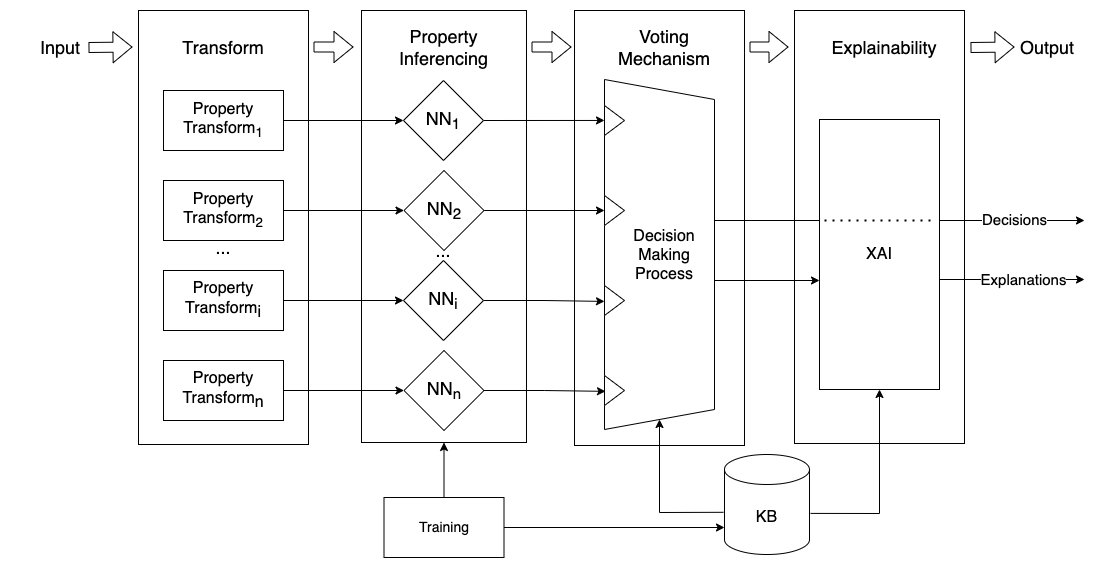
\includegraphics[width=9.2cm]{./images/xai-pipeline.png}
    \caption{Property-Based XAI Data Pipeline}
    \label{fig:xai_data_pipeline}
\end{figure}

The methodology for building the XAI system takes training and test sets as
input. The training and test sets are composed of sets $X$ and $Y$ where $x_j
\in X$ and $y_j \in Y$ represent the sample and label, for the $j^{th}$ item of
the set, respectively.  The sample, $x_j$, from the MNIST and EMNIST datasets
are simply a 28x28 input image and the label, $y_j$, an unsigned 8 bit integer,
representing the class of the corresponding sample. 

The first step of constructing the system is to discover explainable properties.
Samples from the training set are reviewed manually to identify explainable
properties. Explainable properties are characteristics of particular classes of
input samples.

An example of an explainable property comes from an observation that uppercase
characters such as A, E, F, H, I and L often contain line properties. Lines are
an explainable geometric property of some characters. Another explainable
property comes from observing circles or semicircles in letters like O, Q, B, P,
D. Circles and semicircles are, therefore, explainable properties of some
characters. A third property is called stroke.  The stroke represents the
undirected path traced by the writing implement and does not consider the width
which could vary between characters based on the writer, tip of the implement,
or pressure.

From the list of explainable properties, property transforms are identified.  A
property transform is a modification of the input to highlight an explainable
property.  Transform modules implement the conversion of the input to exemplify
traces of the property in the input.

Since line and circle explainable properties were identified in many classes of
characters, it may be beneficial to find a transform that highlights lines and
circles in images.  There is such a transform, the Hough
transform\cite{Hough1959qva}.  A modules are composed to perform a hough
transforms for linear and circle or ellipse features.  The stroke of a character
can be highlighted by taking the morphological skeleton\cite{LEE1994} of the
input image.

After implementing transform modules for each of the properties, test and
training sets must be transformed and prepared for training. NNs are implemented
in a 1:1 relationship with transform modules and trained using the transformed
training set.  A NN is trained on and receives input from one property
transformation.  Each resulting trained NN will make fine-grained inferences
based on its explainable property.

Upon completing the training of the NNs, the Knowledgebase (KB) may be
constructed. This is done by processing the transformed training data by the
NNs and storing the results in the KB along with training labels.  The data in
KB is then used to gauge the effectiveness, $E$, of each property transform and
NN for a particular class.  The effectiveness metrics are stored in the
Knowledgbase and are used to assist in the voting mechanism.

A probabilistic voting scheme is constructed as a module to combine the granular
classification results and utilize the effectiveness metrics to make a set of
global classification decisions and confidence for each decision based on
effectiveness.

Finally, an XAI module is constructed that takes the output of property
inferencing and the global decision from voting to composes an explanation.
This XAI module relates the explainable properties that contributed to a global
decision and bases the explanation on the explainable properties.

Python applications implement the stages of the explainable data pipeline from
Fig.~\ref{fig:xai_data_pipeline}. Modules transform the EMNIST data according to
explainable properties, construct and train the ML models, build the
knowledgebase, implement probabilistic inferencing, and finally a module
constructs the rationale based on properties contributing to the global
decision.

Properties and corresponding property transforms that were utilized consist of:
\begin{itemize}
    \item The stroke property and skeleton transform
    \item The circle property and Hough circle transform
    \item The circle property and multiple non-overlapping Hough circle transforms
    \item The crossing property and the corresponding crossing transform
    \item The ellipse property and the Hough ellipse transform
    \item The endpoint property and the endpoint transform
    \item The enclosed region property and the flood fill transform
    \item The line property and the linear Hough transform
    \item The enclosed region of the stroke and the flood fill of the skeleton
    \item The area property and the convex hull transform
\end{itemize}

A new property added to this methodology is the area property, representing the general
region of the image that a character consumes. The corresponding
property transform is the convex hull. Fig.~\ref{fig:zero_raw} represents an
original zero sample and Fig.~\ref{fig:zero_ch} represents the convex hull
transform of the original zero.

\begin{figure}[h]
    \centering
    \begin{subfigure}{.5\columnwidth}
        \centering
        
\includegraphics[width=3cm]{./images/raw_0-0-12.png}
        \caption{A zero base image}
        \label{fig:zero_raw}
    \end{subfigure}%
    \begin{subfigure}{.5\columnwidth}
        \centering
        
\includegraphics[width=3cm]{./images/ch_0-0-12.png}
        \caption{The convex hull of \ref{fig:zero_raw}}
        \label{fig:zero_ch}
    \end{subfigure}
    \caption{An example of the convex hull transform of the digit zero}
    \label{fig:chull_example}
\end{figure}

The property inferencing phase of the pipeline was implemented in three
different ways to compare performance of differing NN models.  One
implementation used Multi-Layer Perceptrons (MLP), two hidden layers of 128
perceptrons.  The second implementation used a two layer CNN.  The final
implementation used Resnet50 models.

Before using the explainable pipeline, the MLP, CNN, and Resnet50 models were
trained and tested on untransformed data to establish a baseline for
unexplainable recognition.  The results are outlined in Table
\ref{tab_unexplainable accuracy_results}.

After applying the XAI pipeline to the balanced EMNIST dataset, a significant
degradation in accuracy was observed in comparison to the unexplainable results.
After considering opportunities for improving performance, the option of further
splitting the EMNIST dataset by classes was used.  Balanced EMNIST was
split into a dataset consisting of only digits, only uppercase digits (26
classes), and only lowercase letters.  The argument that when letters are
observed in context, among other handwritten letters, it may be apparent from
which split the letter belongs.  After splitting the balanced dataset,
additional unexplainable and explainable baselines were obtained for later
comparison in Sec. \ref{emnist_results}.

\subsection{Explainability Metric for Unexplainable Components}

A strategy for improving the accuracy of the pipeline, at the cost of
explainability, is to add a NN to the inferencing stage that will be trained on
the untransformed sample and treat it as unexplainable in the system.  That
unexplainable contribution would have a high effectiveness metric, because of
its accuracy, and would contribute to confidence but would not contribute to the
explanation.  Consider the system from \cite{whitten21} with all explainable
properties, the properties are treated equally in terms of the explanation. If
an unexplainable component is added, there should be a means of detracting form
the explainability. This may be accomplished by assigning an explainability
component $x_i$ to each NN, $i$.  Explainable NNs would have $1.0 \geq x_i > 0$
while unexplainable would have $x_i = 0$.  The explainable components would be
summed for each class $d$ the NNs vote for to give explainability $X_d$ in
Eq.~\ref{eq:explainability} where $x_{i,d}$ represents the explainable component
from NNs that vote for class $d$ and $V_d$ is the set of NNs that vote for class
$d$.  In such a system, the output of the system would consist of the set of
class, confidence, explainability trips for each potential solution.  Note that
explainability would be $1.0 \geq X_d \geq 0$, with $X_d = 1.0$ signifying that
only explainable NNs voted for $d$ while values $X_d < 1.0$ would signify that a
vote was contributed by an unexplainable NN for class $d$.


\begin{equation}
    X_d=\frac{\sum_i x_{i,d}}{|V_d|}
    \label{eq:explainability}
\end{equation}

\subsection{Removing Ambiguous Data}

In an attempt improve explainable results the removal of ambiguous and
mislabeled data was explored. Data and pruning of the training and test sets
were performed in several ways and compared.

The first pruning scheme was based on a threshold, of 75\% confidence, which
eliminated 5\% of the training set. Results of threshold pruning were observed
on a per class basis and it was noted in Table \ref{tab_threshold_pruning_qty}
that in some classes, over half of the samples were removed.  E.g., for
uppercase letters, the I and L classes had more than 1200 of the 2400 samples
for each class pruned. This pruning caused a highly unbalanced training set and
resulted in only 13\% accuracy on uppercase letters.  Higher thresholds up to
95\% were also attempted, however, poor accuracy results were observed most
likely due to unbalancing the training set.

\begin{table}
    \centering
    %\resizebox{\textwidth}{!}
    \caption{\label{tab_threshold_pruning_qty}The number of pruned samples based on a 75\% confidence threshold}
\end{table}

The second pruning scheme limited the pruning to only the worst 5\% confidence
of each class. Wrong classifications were especially penalized by assigning the
confidence a negative value, via multiplication by $-1.0$.  A negative value on
wrong classifications practically ensures a sample will be pruned. The results on
this pruned training and test set were about 89.24\% accuracy on uppercase letters
versus 86.75\% on unpruned data.  This scheme used a K-fold Cross-validation to
ensure that confidence of the training set samples were attained out of sample
and without bias.

Another means of pruning involved leveraging Cleanlab to remove issues from the data.
Cleanlab was also used iteratively with three passes and results are reviewed in
\ref{emnist_results}.

\section{Results}


%Results for addition of the convex hull are 97.1\% accuracy.  TODO add more details
%here.

%Results for adding the two hidden layer CNN are 96.0\% versus 91.9, a 4\%
%increase on the MNIST dataset from \cite{whitten21}.  TODO: add more here.

\subsection{EMNIST Results}
\label{emnist_results}

Table~\ref{tab_unexplainable accuracy_results} shows the accuracy results using
only the indicated NN on the various EMNIST datasets.  Note that the accuracy
results are only using the base images without transformation and a single NN.
The two layer CNN can be observed as having the top results.  This maybe due to
image resizing that was necessary as the Resnet implementation utilized requires
a minimum input of 32x32.  

\begin{table}
    \centering
    \resizebox{\columnwidth}{!}{%
    \begin{tabular}{|l|c|c|c|c|c|c|c|c|}
        \cline{2-9}
        \multicolumn{1}{c}{} & \multicolumn{8}{|c|}{Accuracy (\%)} \\
        \cline{2-9}
        \multicolumn{1}{c}{} & \multicolumn{2}{|c|}{Full EMNIST} & \multicolumn{2}{|c|}{EMNIST Digits} & \multicolumn{2}{|c|}{EMNIST Caps} & \multicolumn{2}{|c|}{EMNIST Lower} \\
        \hline
        ML Model & Train & Test & Train & Test & Train & Test & Train & Test \\
        \hline
        \hline
        MLP & 82.59 & 78.68 & 99.82 & 97.32 & 95.88 & 91.13 & 97.91 & 89.47 \\
        \hline
        Two layer CNN & 89.14 & 88.66 & 99.44 & 99.05 & 95.87 & 95.36 & 94.84 & 93.41 \\
        \hline
        Resnet50 & 88.69 & 88.68 & 99.44 & 98.90 & 95.26 & 94.89 & 97.07 & 92.68 \\
        \hline
    \end{tabular}
    }
    \caption{\label{tab_unexplainable accuracy_results}Unexplainable accuracy results on various balanced EMNIST data sets with differing NN models}
\end{table}

Table \ref{tab_explainable accuracy_results} shows the explainable accuracy
results on the unpruned data. Compared to Table \ref{tab_unexplainable
accuracy_results} the results are lower.  As expected, there appears to be a
cost in decreased accuracy for explainability as implemented in this
methodology. %TODO: add more details here.

The Resnet50 models appeared to perform better with the uppercase letters.  The
uppercase letter dataset had 2.5 times the number of classes as the other data
sets, 26 classes versus 10.  It should be noted that on the full balanced
dataset with 46 classes Resent50 and the CNN performed nearly identically. 

\begin{table}
    \centering
    \resizebox{\columnwidth}{!}{%
    \begin{tabular}{|l|c|c|c|c|c|c|c|c|}
        \cline{2-9}
        \multicolumn{1}{c}{} & \multicolumn{8}{|c|}{Accuracy (\%)} \\
        \cline{2-9}
        \multicolumn{1}{c}{} & \multicolumn{2}{|c|}{Full EMNIST} & \multicolumn{2}{|c|}{EMNIST Digits} & \multicolumn{2}{|c|}{EMNIST Caps} & \multicolumn{2}{|c|}{EMNIST Lower} \\
        \hline
        ML Model & Train & Test & Train & Test & Train & Test & Train & Test \\
        \hline
        \hline
        MLP & 71.04 & 64.99 & 95.10 & 90.80 & 81.22 & 73.81 & 91.68 & 81.41 \\
        \hline
        Two layer CNN & 68.21 & 64.97 & 93.63 & 92.65 & 80.10 & 79.96 & 88.77 & 86.57 \\
        \hline
        Resnet50 & 87.06 & 73.93 & 93.10 & 91.86 & 90.79 & 86.75 & 79.10 & 81.30 \\
        \hline
    \end{tabular}
    }
    \caption{\label{tab_explainable accuracy_results}Explainable accuracy results on various balanced EMNIST data sets with differing NN models}
\end{table}

Table~\ref{raw_cap_confusion_matrix} shows the confusion matrix for interesting
uppercase letters after running though the explainable pipeline. There is
significant confusion with the I and L classes and a fair degree of confusion
with the U and V classes.

%\begin{figure}[h]
%    \centering
%    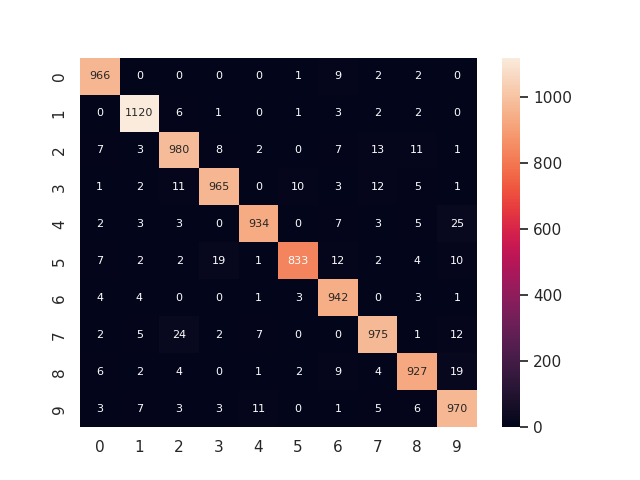
\includegraphics[width=10cm]{./images/confusion_matrix_vlsid.png}
%    \caption{Confusion matrix using convex hull}
%    \label{fig:conf_matrix}
%\end{figure}

\begin{table}
    \centering
    %\resizebox{\columnwidth}{!}{%
    \begin{tabular}{ |c|c|c|c|c|c|c|c|c|}
    \hline
     & H & I & J & K & L & M & U & V \\
    \hline
    H & 374 &  & 1 & 3 &  & 11 & 1 & 1 \\
    \hline
    I &  & 275 & 2 & & 114 & & & \\
    \hline
    J &  & 11 & 376 & & 1 & & 2 & 6 \\
    \hline
    K &  &  &  & 392 & 1 & & & \\
    \hline
    L &  & 90 &  &  & 306 & & & \\
    \hline
    M &  &  &  &  &  & 399 & & 1 \\
    \hline
    U & 4 & 1 & & 1 & 9 & & 305 & 29 \\
    \hline
    V & & & 2 & & 2 & 2 & 9 & 326 \\
    \hline
    \end{tabular}
    %} 
    \caption{\label{raw_cap_confusion_matrix}Explainable confusion matrix for unpruned uppercase letters H - M, U, and V}
\end{table}

After applying one round of Cleanlab to prune only training labels with issues,
Table \ref{raw_cap_cleanlab_confusion_matrix} indicates the same uppercase
letters of interest. The confusion in the I class appears to have gotten better.
L, U, and V classes appear to have gotten worse. Six of the eight classes of
interest had decreases in correct classifications, the values along the
diagonal.  Using CNNs, the overall results of one round of Cleanlab were
decrease in accuracy to 87.4\% on uppercase letters from 88.7\% without pruning.

\begin{table}
    \centering
    %\resizebox{\columnwidth}{!}{%
    \begin{tabular}{ |c|c|c|c|c|c|c|c|c|}
    \hline
    ~ & H & I & J & K & L & M & U & V \\
    \hline
    H & 368 & & 1 & 2 & & 7 & 1 & \\
    \hline
    I &  & 293 & 4 &  & 65 & 14 & & \\
    \hline
    J & & 17 & 339 & & 1 & 6 & 1 & 2 \\
    \hline
    K & 5 &  &  & 349 & 2 & 20 &  & \\
    \hline
    L & 0 & 120 &  & 1 & 236 & 2 & & \\
    \hline
    M & 4 & & & 3 & & 383 & & \\
    \hline
    U & 2 & & 1 & 1 & & 22 & 304 & 17 \\
    \hline
    V & & & 3 & 1 & & 21 & 13 & 315 \\
    \hline
    \end{tabular}
    %}
    \caption{\label{raw_cap_cleanlab_confusion_matrix}Explainable confusion matrix for
    uppercase letters H - M, U, and V after a single cleanlab pruning}
\end{table}

After applying subsequent rounds of Cleanlab to the capital letter dataset, the
accuracy returned to 88.7\% after the third iteration of pruning. Table
\ref{raw_cap_cleanlab_third_confusion_matrix} again shows the confusion matrix
for the classes of interest after the third Cleanlab pruning.

\begin{table}
    \centering
    %\resizebox{\columnwidth}{!}{%
    \begin{tabular}{ |c|c|c|c|c|c|c|c|c|}
    \hline
    ~ & H & I & J & K & L & M & U & V \\
    \hline
    H & 357 & &  & 8 & & 2 & 1 & 1 \\
    \hline
    I &  & 254 & 3 & 3 & 101 & 1 & & \\
    \hline
    J & & 19 & 298 & 1 & 16 & & 2 & 6 \\
    \hline
    K & 3 &  &  & 352 & 2 & 2 & 0 & \\
    \hline
    L & 0 & 90 & 1 & 1 & 277 & & & \\
    \hline
    M & & & & 3 & & 378 & & 1 \\
    \hline
    U & 1 & & 1 & 9 & & 1 & 305 & 29 \\
    \hline
    V & & 2 & & 2 & 2 & 1 & 9 & 326 \\
    \hline
    \end{tabular}
    %}
    \caption{\label{raw_cap_cleanlab_third_confusion_matrix}Explainable confusion matrix for
    uppercase letters H - M, U, and V after three rounds of Cleanlab pruning}
\end{table}


\subsection{Explainability Results}

%We can show that since we are using the probabilistic voting that explainability quality is 100\%.
%Can we introduce other metrics?

This section depicts the explainability results using examples from the EMNIST
balanced test set.  Example 1, which is labeled as an uppercase Q, is shown in
Fig.~\ref{fig:ex1}.  Table \ref{table:example1} shows that votes for classes Q,
Z, R, and D were made by various properties.  Six of the properties contributed
a vote for Q and one property each voted on the other classes.  Summing the
effectiveness weights for the classes, Q wins with a confidence of 71\%.

\begin{figure}
    \centering
    
\includegraphics[width=3cm]{./images/examples/test-Q-0.png}
    \caption{Example 1: a test sample labeled Q}
    \label{fig:ex1}
\end{figure}

\begin{table}
    \caption{Prob. voting, effectiveness, and explainability for example 1}
    \centering
    \resizebox{\columnwidth}{!}{%
    \begin{tabular}{| c | c | c | c | c | c | c | c | c | c | c |}
    \cline{4-11}
    \multicolumn{3}{c}{} & \multicolumn{4}{|c|}{Effectiveness} & \multicolumn{4}{c|}{Explainability} \\
    \hline
     $P_j$ & Property & Vote & $E_{j,Q}$ & $E_{j,Z}$ & $E_{j,R}$ & $E_{j,D}$ & $X_Q$ & $X_Z$ & $X_R$ & $X_D$ \\
    \hline \cline{0-10}
    $P_0$ & Stroke & Q & 0.96 &  &  &  & \checkmark &  &  & \\ 
    \hline
    $P_1$ & Circle & Q & 0.57 &  &  &  & \checkmark &  &  &  \\
    \hline
    $P_2$ & Crossing & D &  &  &  & 0.36 &  &  &  & \checkmark \\
    \hline
    $P_3$ & Circle & Q & 0.43 &  &  &  & \checkmark &  &  &  \\
    \hline
    $P_4$ & Circle & Q & 0.63 &  &  &  & \checkmark &  &  &  \\
    \hline
    $P_5$ & Endpoint & Z &  & 0.56 & &  &  & \checkmark &  &  \\
    \hline
    $P_6$ & Encl. Reg. &  &  &  &  &  &  &  &  &  \\
    \hline
    $P_7$ & Line & R &  &  & 0.50 &  &  &  & \checkmark &  \\
    \hline
    $P_8$ & Encl. Reg. & Q & 0.70 &  &  &  & \checkmark &  &  &  \\
    \hline
    $P_9$ & Area & Q & 0.98 &  &  &  & \checkmark &  &  &  \\
    \hline \cline{0-10}
    \multicolumn{3}{|c|}{Weight} & 3.73 & 0.56 & 0.46 & 0.27 & \multicolumn{4}{c|}{$\sum W_k=5.26$} \\
    \cline{0-10}
    \multicolumn{3}{|c|}{Confidence} & $71\%$ & $15\%$ & $9\%$ & $5\%$ & \multicolumn{4}{c}{} \\
    \cline{0-6}
    \end{tabular}%
    }
    \label{table:example1}
\end{table}

Explainable rationale provided by XAI is depicted in \ref{table:exexample1} for the four classes that
received votes from the NNs.  Along with the classes and confidence levels from Table \ref{table:example1}
the explanations are output from the system.

\begin{table}
    \caption{Rationale for example 1}
    \centering
    \begin{tabular}{| p{0.04\linewidth} | p{0.14\linewidth} | p{0.65\linewidth} |}
    \hline
     $X_d$ & Confidence & Explainable Description \\
    \hline \cline{1-3}
    $X_Q$ & 71\% & Confidence is high for interpreting as a Q due to the circle, stroke, area, and enclosed region properties. \\ 
    \hline
    $X_Z$ & 15\% & Confidence is low for interpreting as a Z due to endpoint properties. \\
    \hline
    $X_R$ & 9\% & Confidence is low for interpreting as a R due to line properties. \\
    \hline
    $X_D$ & 5\% & Confidence is low for interpreting as a D due to crossing properties. \\
    \hline
    \end{tabular}
    \label{table:exexample1}
\end{table}

Figure \ref{fig:ex2} shows example two from the test set which is labeled as an
uppercase C. Votes by the properties in Table \ref{table:example2} show that
several properties infer an uppercase C, e.g., stroke, endpoint, area, circle,
and crossing. The overall weight for the class C is 4.95 from the effectiveness
of the properties giving it a confidence of 74\%. The uppercase Z receives a
vote from the enclosed region property. Uppercase O receives a vote from the
circle property via the ellipse transform.

\begin{figure}
    \centering
    
\includegraphics[width=3cm]{./images/examples/test-C-1.png}
    \caption{Example 2: A test sample labeled C}
    \label{fig:ex2}
\end{figure}

\begin{table}
    \caption{Prob. voting, effectiveness, and explainability for example 2}
    \centering
    \resizebox{\columnwidth}{!}{%
    \begin{tabular}{| c | c | c | c | c | c | c | c | c |}
    \cline{4-9}
    \multicolumn{3}{c}{} & \multicolumn{3}{|c|}{Effectiveness} & \multicolumn{3}{c|}{Explainability} \\
    \hline
     $P_j$ & Property & Vote & $E_{j,C}$ & $E_{j,Z}$ & $E_{j,O}$ & $X_C$ & $X_Z$ & $X_O$ \\
    \hline \cline{0-8}
    $P_0$ & Stroke & C & 1.0 &  &  & \checkmark &  & \\ 
    \hline
    $P_1$ & Circle & C & 0.37 &  &  & \checkmark &  &  \\
    \hline
    $P_2$ & Crossing & C & 0.12 &  &  & \checkmark &  &  \\
    \hline
    $P_3$ & Circle & C & 0.42 &  &  & \checkmark &  &  \\
    \hline
    $P_4$ & Circle & O &  &  & 0.40 &  &  & \checkmark \\
    \hline
    $P_5$ & Endpoint & C & 0.95 &  &  & \checkmark &  &  \\
    \hline
    $P_6$ & Encl. Reg. & Z &  & 0.10 &  &  & \checkmark &  \\
    \hline
    $P_7$ & Line & C & 0.38 &  &  & \checkmark &  &  \\
    \hline
    $P_8$ & Encl. Reg. &  &  &  &  &  &  &  \\
    \hline
    $P_9$ & Area & C & 0.86 &  &  & \checkmark &  &  \\
    \hline \cline{0-8}
    \multicolumn{3}{|c|}{Weight} & 4.95 & 0.97 & 0.72 & \multicolumn{3}{c|}{$\sum W_k=6.64$} \\
    \cline{0-8}
    \multicolumn{3}{|c|}{Confidence} & $74\%$ & $15\%$ & $11\%$ & \multicolumn{3}{c}{} \\
    \cline{0-5}
    \end{tabular}%
    }
    \label{table:example2}
\end{table}

\begin{table}
    \caption{Rationale for example 2}
    \centering
    \begin{tabular}{| p{0.04\linewidth} | p{0.14\linewidth} | p{0.65\linewidth} |}
    \hline
     $X_d$ & Confidence & Explainable Description \\
    \hline \cline{1-3}
    $X_C$ & 74\% & Confidence is high for interpreting as a C due to the stroke, endpoint, area, circle, and crossing properties. \\ 
    \hline
    $X_Z$ & 15\% & Confidence is low for interpreting as a Z due to enclosed region properties. \\
    \hline
    $X_O$ & 11\% & Confidence is low for interpreting as a O due to circle properties. \\
    \hline
    \end{tabular}
    \label{table:exexample2}
\end{table}

The vote for an uppercase Z for example 2 by the enclosed region is a bit
confusing as there should be no resulting enclosed pixels in the transformed C,
i.e., a flood fill, which is the transform associated with the enclosed region,
should result in no pixels in the output image since a C has no enclosed region.
A review of the resulting transform shows that this is indeed the case.  Test
results show that samples form several classes, such as Y and L, that would not
have pixels in a flood fill get Z votes from the enclosed region property.  This
suggests that an improvement in the system could be to discount results from
transforms void of any activated pixels, especially when the transform has
several classes that generate empty images, due to the lack of a particular
property.  Improvements could also be accomplished using knowledge of the
explainable properties associated and not associated with each class.
Implementing such rules into the pipeline add elements of an expert system and
detract from the generality of the XAI system.

Table \ref{table:exexample2} shows the explainability for example 2.  In this case, the system indicates:

\begin{itemize}
    \item Confidence is high for interpreting as a C due to the stroke, endpoint, area, circle, and crossing properties.
    \item Confidence is low for interpreting as a Z due to enclosed region properties.
    \item Confidence is low for interpreting as a O due to circle properties.
\end{itemize}

\subsection{Inferencing Mislabeled Pruned Data}

Images pruned from the training set due to issues such as mislabeled or
ambiguous samples after one Cleanlab pruning were submitted back to the system.  
Of the 1188 pruned images only 129 or about 11\% of the problematic labels from
the original training set were recognized as correctly labeled.  The remaining
89\% were still unrecognizable and still ambiguous as to the class. Some of the
pruned images are depicted in Fig.~\ref{fig:pruned_inf_samples}.  In many cases
the XAI pipeline was able to correctly inference mislabeled samples.

\begin{figure}[h]
    \centering
    \textbf{Pruned Samples}\par\medskip 
    \begin{subfigure}{.20\columnwidth}
        \centering
        
\includegraphics[width=.90\textwidth]{./images/issues/excluded-G-0-inferred-S.png}
        \caption{G label}
        \label{fig:inf_issue_G0}
    \end{subfigure}%
    \begin{subfigure}{.20\columnwidth}
        \centering
        
\includegraphics[width=.90\textwidth]{./images/issues/excluded-T-5-inferred-u.png}
        \caption{T label}
        \label{fig:inf_issue_T5}
    \end{subfigure}%
    \begin{subfigure}{.20\columnwidth}
        \centering
        
\includegraphics[width=.90\textwidth]{./images/issues/excluded-O-7-inferred-M.png}
        \caption{O label}
        \label{fig:inf_issue_O7}
    \end{subfigure}%
    \begin{subfigure}{.20\columnwidth}
        \centering
        
\includegraphics[width=.90\textwidth]{./images/issues/excluded-W-3-inferred-M.png}
        \caption{W label}
        \label{fig:inf_issue_W3}
    \end{subfigure}%
    \begin{subfigure}{.20\columnwidth}
        \centering
        
\includegraphics[width=.90\textwidth]{./images/issues/excluded-O-10-inferred-F.png}
        \caption{O label}
        \label{fig:inf_issue_O10}
    \end{subfigure}
    \caption{Pruned samples that were inferred by the system.
    Fig.~\ref{fig:inf_issue_G0}, originally labeled as a G was inferred correctly as an S with 42\% confidence.
    Fig.~\ref{fig:inf_issue_T5}, originally labeled as a T was inferred correctly as a U with 36\% confidence.
    Fig.~\ref{fig:inf_issue_O7}, originally labeled as an O was inferred correctly as an M with 56\% confidence.
    Fig.~\ref{fig:inf_issue_W3}, originally labeled as a W was inferred correctly as an M with 65\% confidence.
    Fig.~\ref{fig:inf_issue_O10}, originally labeled as an O was inferred correctly as an F with 40\% confidence.
    }
    \label{fig:pruned_inf_samples}
\end{figure}

Clearly the quality of the training set is a big concern with NN and XAI.  The
pruning methods we present attempts to improve the quality of the training set
to enhance accuracy and explainability. The XAI pipeline benefits in two ways,
(a) it was able to correct the problematic, pruned labels with a good degree of
confidence, in some cases (b) the XAI pipeline provided rationale based on
explainable properties that could help a user resolve issues with labels.

\section{Conclusion}

%Achieved acceptable accuracy results.  Explainability based on properties and trust in the system.

%Cost in accuracy for explainability.

%The XAI pipeline was able to inference mislabeled samples.

%TODO: add more.

%This paper introduces a neural network architecture which recognizes handwritten characters and produces explanations based on a character property analysis.

This paper introduced an XAI data pipeline for recognizing handwritten
characters. This work identified and pruned issues in the EMNIST dataset.  The
XAI pipeline was used to resolve some of the issues by leveraging
classifications and explanations.  A key concept to explainability that is
introduced here is correctly pruning the training set in order to improve the
explainability and avoid misleading training set labels. Results from the EMNIST
character database are provided.

\bibliographystyle{plain}
\bibliography{references}

\end{document}
